\chapter{Servidor}

O servidor é o software embarcado no HPS do Soc. Ele é o responsável por gerenciar a comunicação entre a interface de rede por onde recebe os dados provenientes do pacote ROS (cliente) e o FPGA\@. A primeira etapa a ser concluída no desenvolvimento do servidor é compilação de uma versão linux para processadores ARM que será instalada no kit de desenvolvimento. O fluxo de boot do linux na placa é resumido na Figura~\ref{fig:linux}. 

\begin{figure}[ht]
	\caption{Boot linux embarcado}
	\begin{center}
		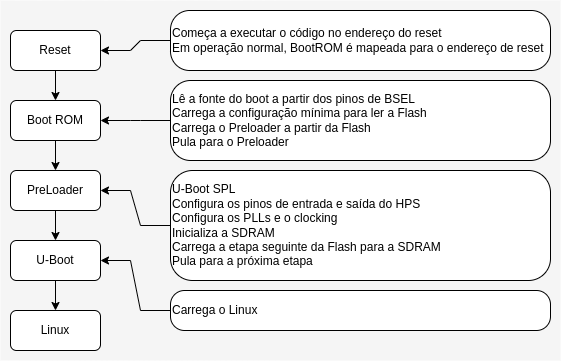
\includegraphics[scale=0.7]{imagens/embeddedLinux.png}\\
		{\small \textbf{Fonte:}\cite{SocLinux}}
    \end{center}\label{fig:linux}
\end{figure}

O primeiro elemento de software é o \textit{Boot ROM} que está gravado de fábrica internamente no dispositivo. Os arquivos de \textit{PreLoader},\textit{ U-boot} e do sistemas de aquivos do linux são salvos em um cartão de memória micro SD\@.

O \textit{Secondary Program Loader - SPL}, conhecido como \textit{PreLoader}, é executado a partir da Boot ROM\@. Ele é responsável por configurar o sistema para que o \textit{bootloader} (U-boot) possa ser executado. A Intel fornece uma ferramenta chamada BSP editor que, a partir de arquivos que descrevem o hardware, podem gerar o PreLoader para o projeto específico~\cite{SocLinux}.  

A etapa seguinte ao \textit{PreLoader} é o \textit{bootloader}. Nessa fase do boot todas as questões de baixo nível do SoC, como por exemplo, os clocks, pinos e SDRAM, já foram inicializados e estão prontos. O objetivo do bootloader, é obter essas informações do sistema e fazer com que ele funcione até o ponto onde o linux possa ser iniciado. Outra função importante do U-boot em um SoC Intel é programar o FPGA~\cite{SocLinux}.




Com o linux já devidamente configurado, ele já pode ser inicializado no processador do SoC, assim podemos iniciar o desenvolvimento do servidor. No primeiro momento devemos realizar o download do código fonte da biblioteca de comunicação, a libinterfacesocket, que já foi detalhada anteriormente, o código fonte pode ser baixado em~\cite{interface-socket-server}. Com os arquivos já no sistema de diretórios do SoC devemos realizar a compilação e a instalação da libinterfacesocket, só assim o servidor terá acesso a suas funcionalidades. 

O acesso do servidor ao FPGA é feito através de mapeamento de endereços do linux, os SoCs Intel possuem uma arquitetura de memória mapeada. Desta forma, além da biblioteca desenvolvida durante a pesquisa, um outro arquivo cabeçalho é necessário para facilitar o acesso aos endereços de memória do HPS\@. Quando uma instância do processador ARM é incluída no projeto do QSys Designer, é gerado um arquivo.sopcinfo no momento em que o projeto é compilado. Podemos usar esse arquivo como entrada da ferramenta \textit{sopc-create-header-files} presente no SoC EDS para gerar um novo arquivo com extensão \textit{.h}, que lista os endereços base de todos os módulos (IP) incluídos no FPGA\@. Portanto, o arquivo cabeçalho gerado disponibiliza o \textit{offset} do endereço em que cada periférico está localizado para cada uma das FPGA-bridges disponíveis. Deste modo o servidor pode enviar ou receber dados ao periférico conhecendo o endereço da FPGA-bridge em que este periférico está conectado e o seu nome, sem a necessidade de se conhecer exatamente o seu endereço.






O Servidor mantém porta aberta para estabelecer uma conexão com o cliente e assim que a conexão é estabelecida, o cliente já pode começar a enviar os dados. Ao receber os dados do cliente, o servidor envia-os ao FPGA que os processa e os devolve ao servidor para que ele possa reenviar os dados já processados ao cliente. Um fluxograma simplificado desse processo pode ser visualizado na Figura \ref{fig:fluxoServidor}.



\begin{figure}[ht]
	\caption{Fluxograma simplificado do servidor}
	\begin{center}
		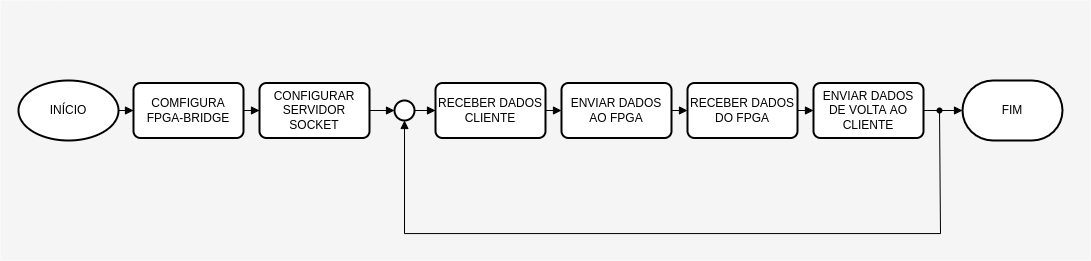
\includegraphics[scale=0.47]{imagens/fluxogramaServidor.png}\\
		{\small \textbf{Fonte:}Elaborado pelo autor}
    \end{center}\label{fig:fluxoServidor}
\end{figure} 
